\section{Evaluación Experimental}
\subsection{Funciones Propuestas por GenOpt}
\begin{frame}
\frametitle{Funciones propuestas por GenOpt}
\begin{block}{Caracteristicas}
\textit{GenOpt} ha propuesto un total de \textbf{18 funciones} de dimensiones $D = 10, 30$ a optimizar, realizando \textbf{cien ejecuciones independientes} para cada una de ellas.
\end{block}
\begin{block}{Familias de Funciones}
\begin{itemize}
	\item Funciones GKLS.
	\item Funciones Clásicas Transformadas.
	 \begin{itemize}
    	\item Rastrigin, $D = 10, 30$ 
    	\item Rosenbrock, $D = 10, 30$ 
    	\item Zakharov, $D = 10, 30$ 
    \end{itemize}
	\item Funciones Compuestas.
	 \begin{itemize}
    	  	\item Goldstein-Price.
    	  	\item Hartmann. 
    	  	\item Sphere.
    	  \end{itemize}
\end{itemize}
\end{block}
\end{frame}

%++++++++++++++++++++++++++++++++++++++++++++++++++++++++++++++++++++++++++++++
\subsection{Estudio de la Parametrización y Rendimiento}

\begin{frame}
\frametitle{Estudio de la Parametrización}
\begin{block}{Objetivos del Estudio}
Determinar los mejores valores para los parámetros de cada algoritmo buscando obtener el máximo rendimiento de cada uno de ellos.
\end{block}
\begin{block}{Poblaciones}
\begin{itemize}
	\item $popsize = 20, 50, 75, 100$ para OBL-CPSO y CMA-ES.
	\item $popsize = 1$ para HSAGS.
	\end{itemize}
\end{block}
\end{frame}

\begin{frame}
\frametitle{Rendimiento de OBL-CPSO}
\begin{figure}
  \centering
	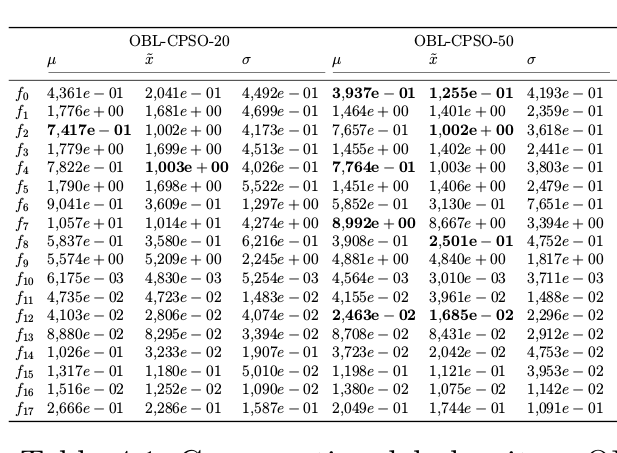
\includegraphics[scale=0.5]{img/oblcpso1}
\end{figure}
\end{frame}

\begin{frame}
\frametitle{Rendimiento de OBL-CPSO}
\begin{figure}
  \centering
	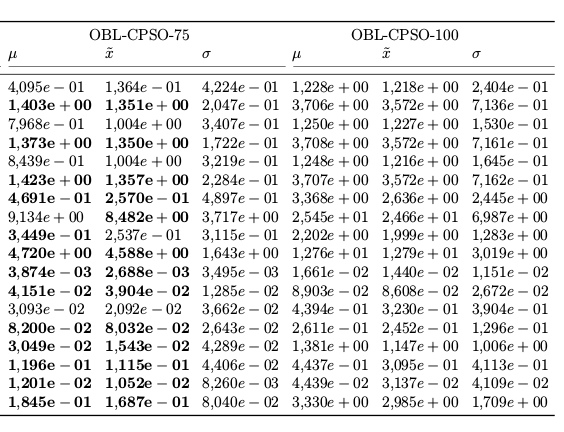
\includegraphics[scale=0.5]{img/oblcpso2}
\end{figure}
\end{frame}

\begin{frame}
\frametitle{Rendimiento de CMA-ES}
\begin{figure}
  \centering
	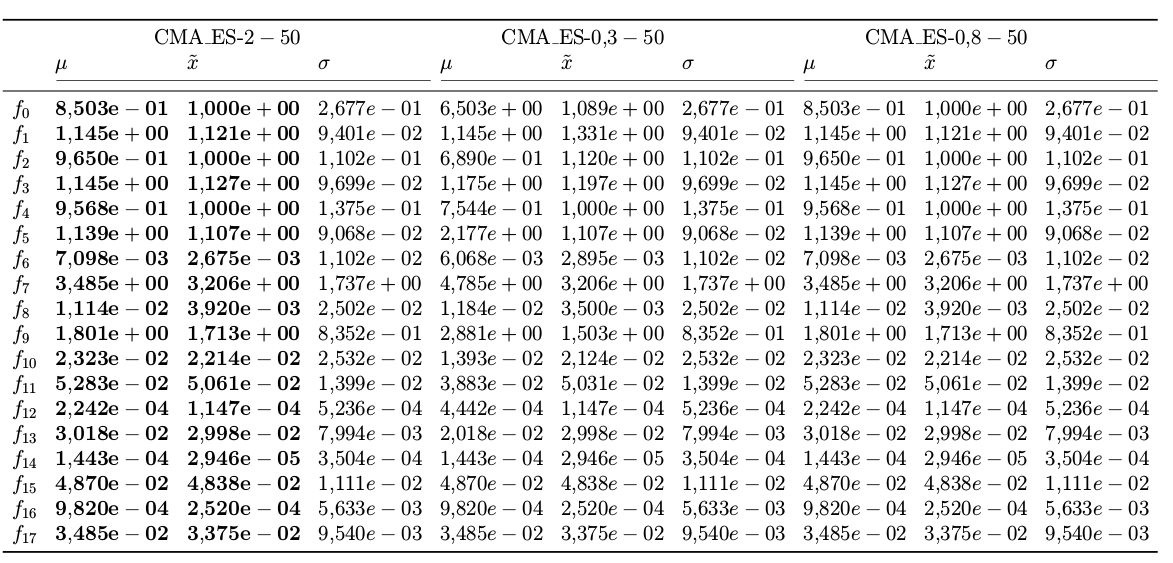
\includegraphics[scale=0.3]{img/cmaF}
\end{figure}
\end{frame}

\begin{frame}
\frametitle{Rendimiento de HSAGS}
\begin{figure}
  \centering
	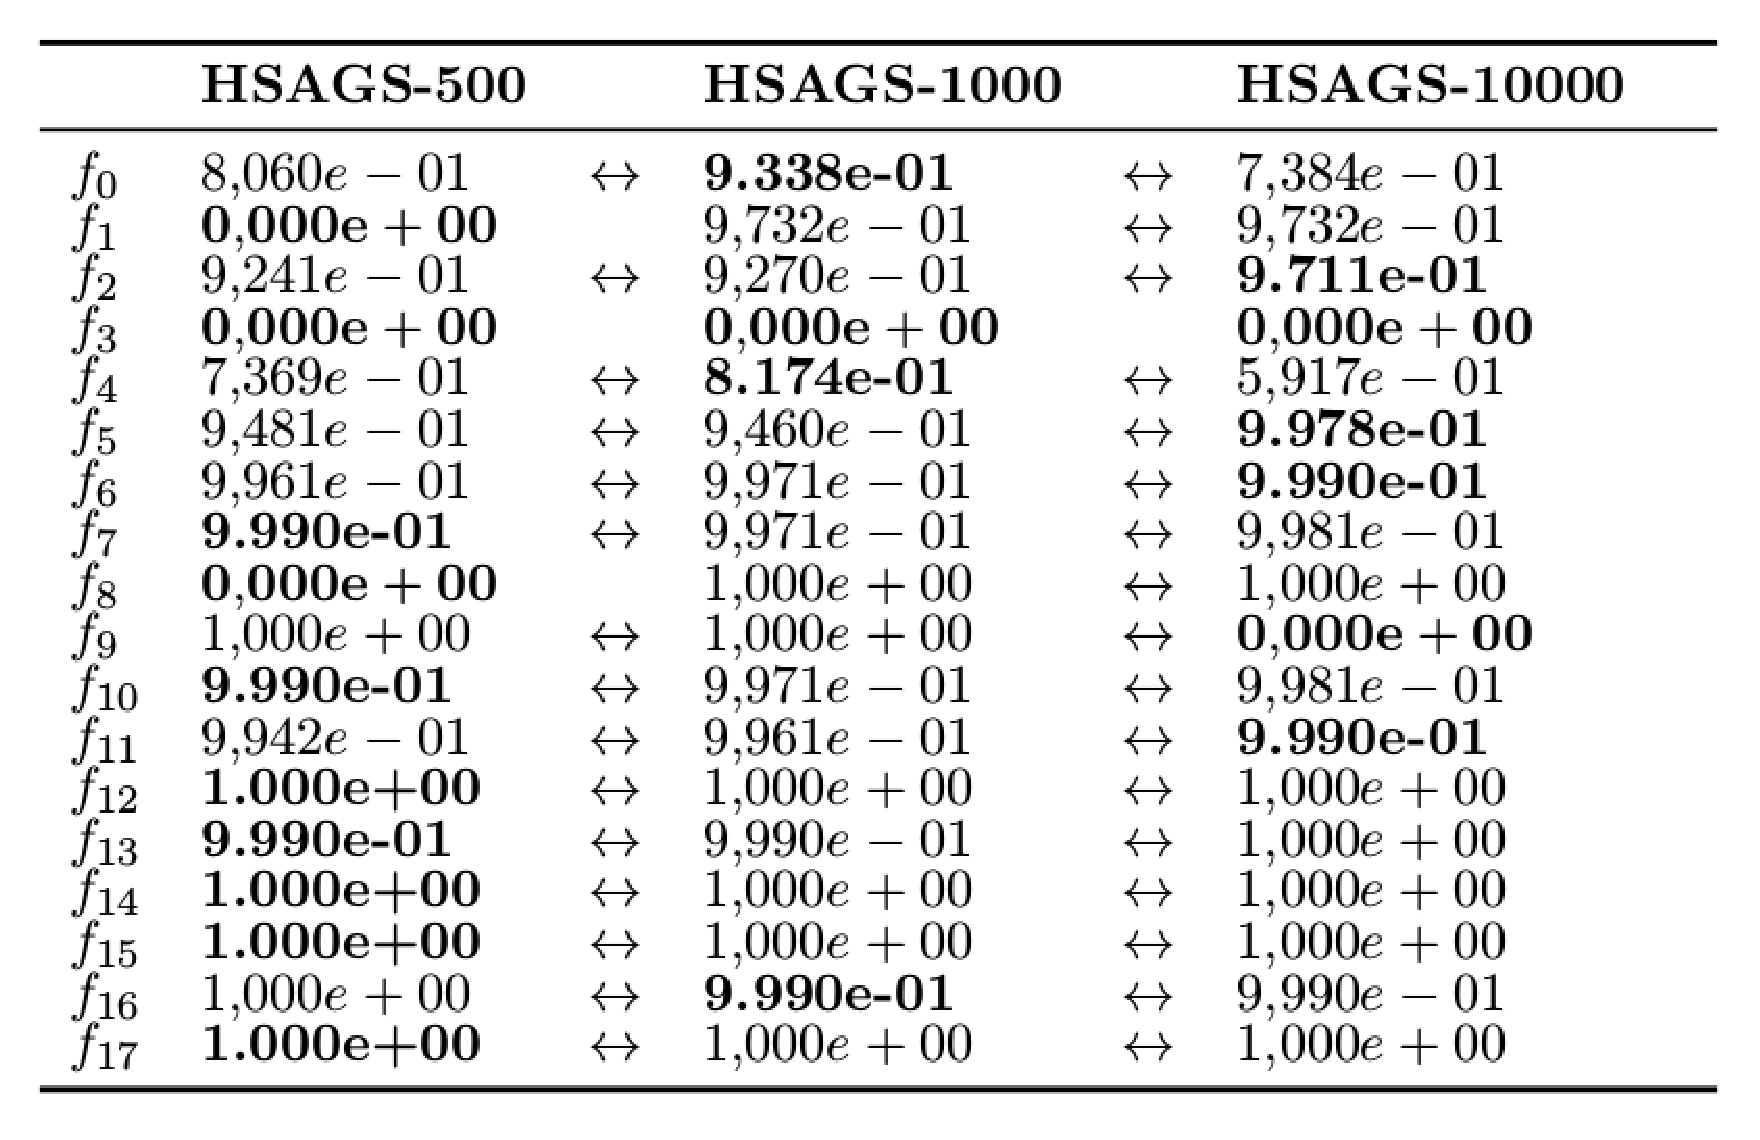
\includegraphics[scale=0.4]{img/hsags}
\end{figure}
\end{frame}

%++++++++++++++++++++++++++++++++++++++++++++++++++++++++++++++++++++++++++++++
\subsection{Comparativa de Rendimiento entre Algoritmos}
\begin{frame}
\frametitle{Comparativa de Rendimiento entre Algoritmos}
\begin{block}{Objetivos del Estudio}
Comparar el rendimiento de cada uno de los algoritmos a la hora de optimizar las funciones propuestas por GenOpt.
\end{block}
\end{frame}

\begin{frame}
\frametitle{Comparativa de Rendimiento entre Algoritmos}
\begin{figure}
  \centering
	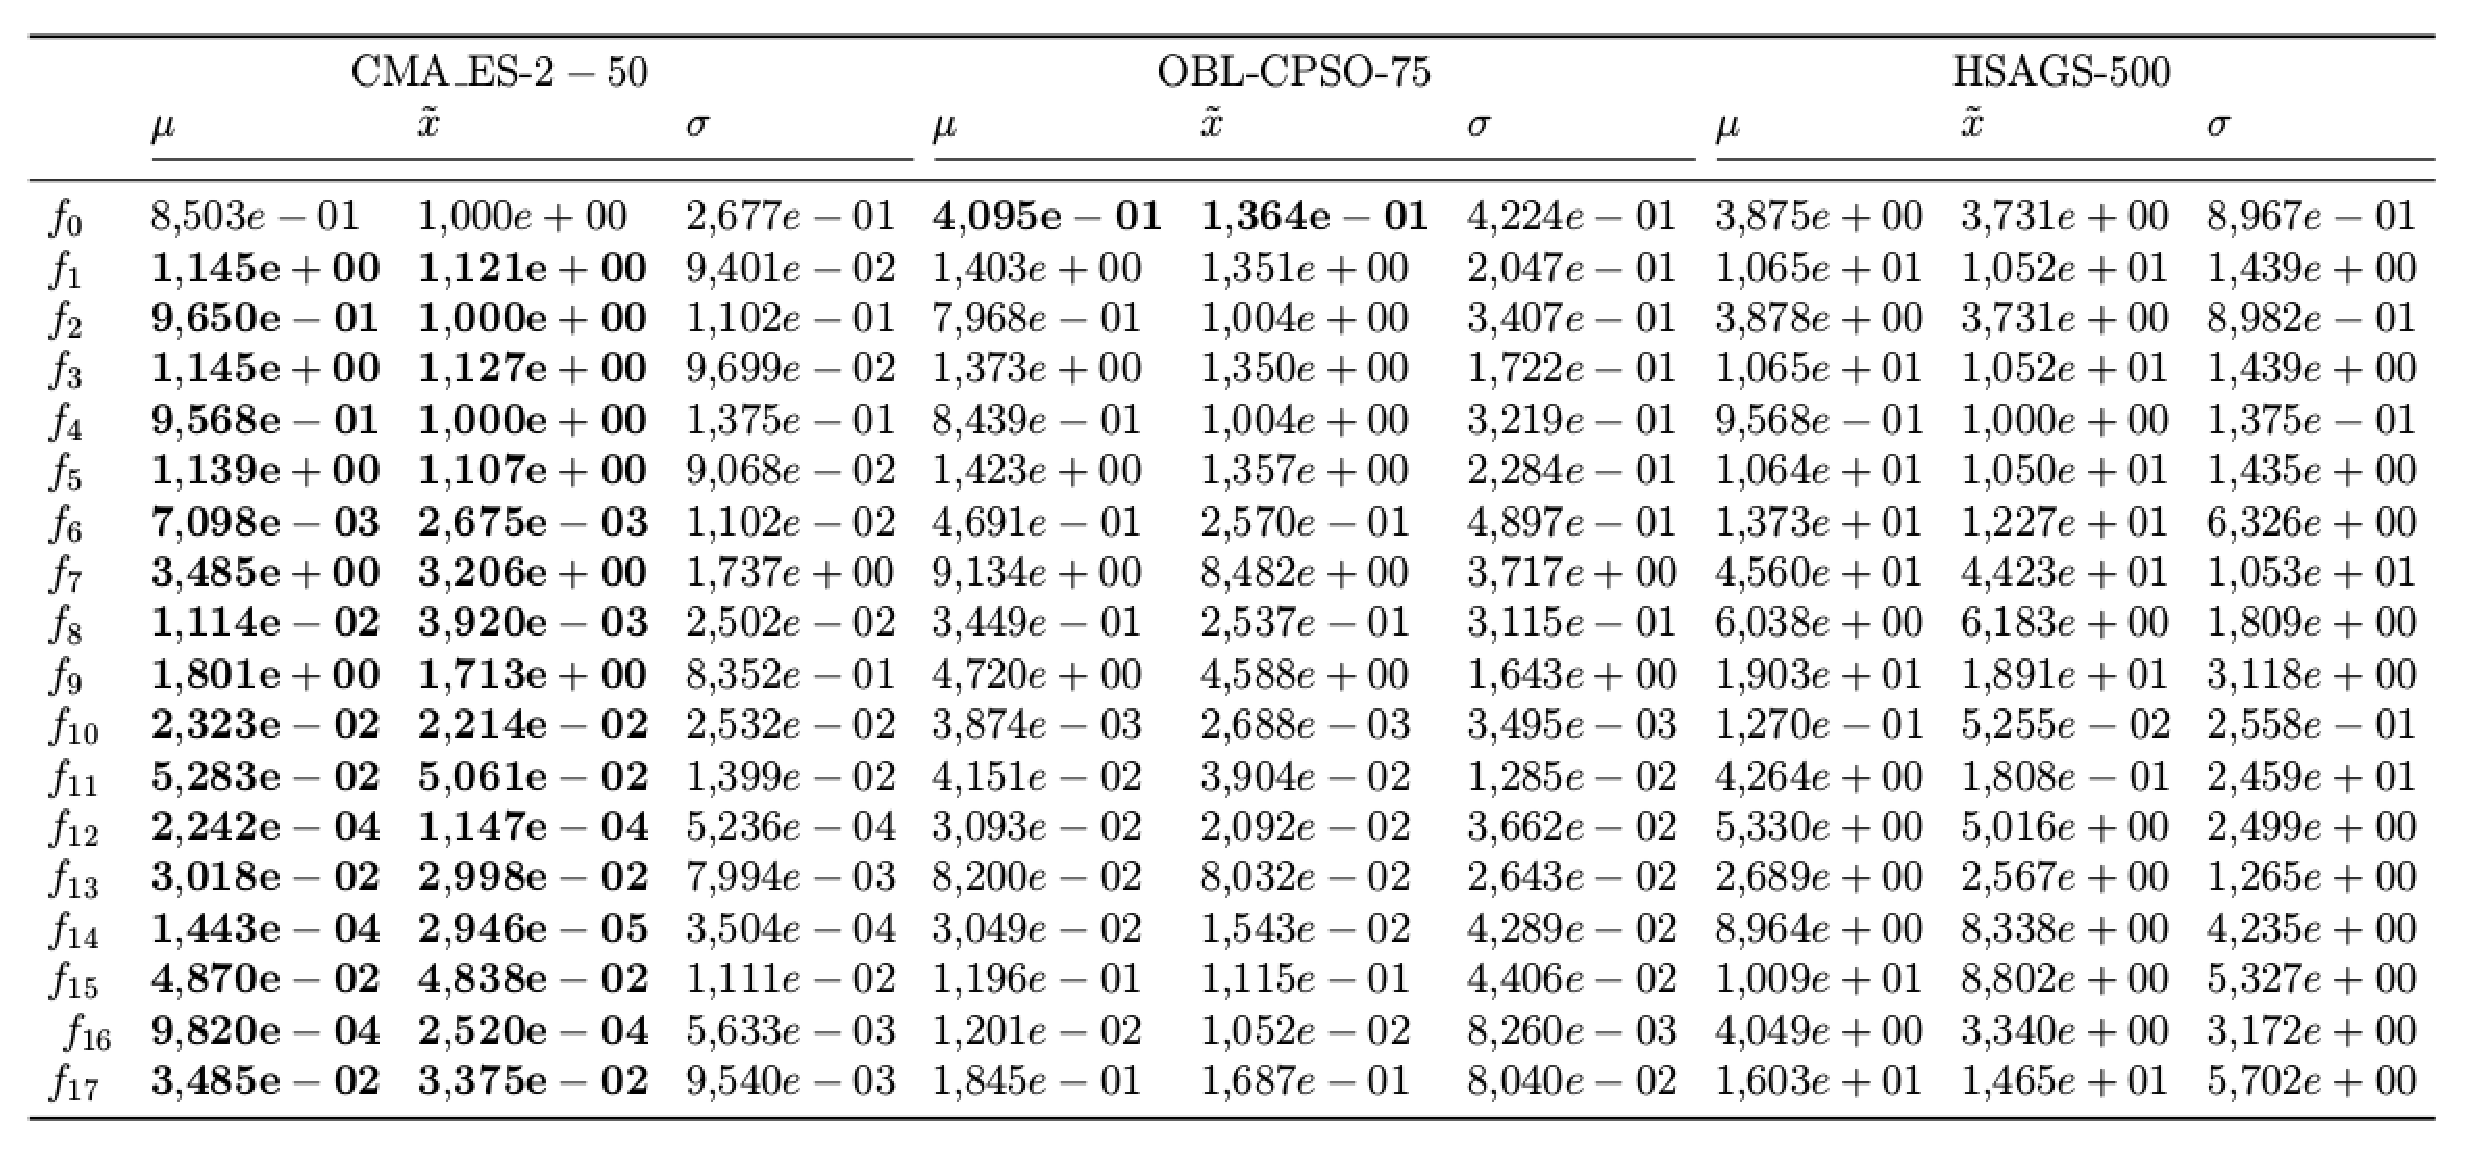
\includegraphics[scale=0.3]{img/finalcmp}
\end{figure}
\end{frame}

%++++++++++++++++++++++++++++++++++++++++++++++++++++++++++++++++++++++++++++++
\subsection{Clasificación en el Concurso GenOpt}
\begin{frame}
\frametitle{Clasificación en el Concurso GenOpt}
\begin{block}{Criterios de Clasificación de GenOpt}
\begin{itemize}
    	  	\item \textbf{High Jump}: mejor valor obtenido en los puntos de control.
    	  	\item \textbf{Target Shooting}: éxito a la hora de alcanzar el óptimo global de la función.
    	  	\item \textbf{Biathlon Score}: media entre el High Jump y Target Shooting.
\end{itemize}
\end{block}
\footnotetext[1]{Manifesto del concurso GenOpt: http://www.genopt.org/genopt.pdf.}
\end{frame}

\begin{frame}
\frametitle{Clasificación en el Concurso GenOpt}
\begin{figure}[!ht]
  \centering
  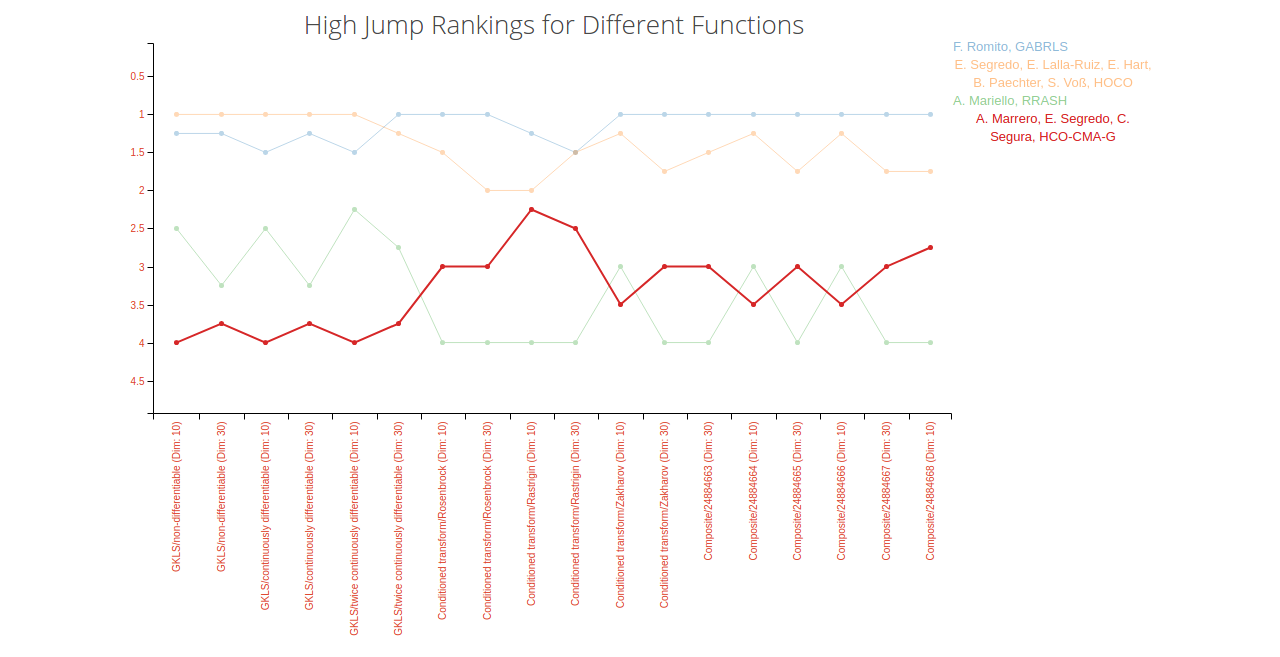
\includegraphics[scale=0.3]{img/highjump}
\end{figure}
\end{frame}